\section{Zielsetzung}
\label{sec:Zielsetzung}

In diesem Versuch soll die Wellenlänge eines Lasers mithilfe des Michelson-Interferometer bestimmt werden.
Ebenso soll der Brechungsindex von Luft bestimmt werden.


\section{Theorie}
\subsection{Interferenz und Kohärenz von Licht}
Die Ausbreitungssvorgänge von Licht lassen sich gut mit der Annahme, dass es sich bei Licht um eine elektromagnetische Welle handelt, beschreiben.
Aus dieser Annahme folgt durch die Maxwell'schen Gleichungen, dass mehrere Lichtstrahlen durch Superposition überlagert werden können.
Der elektrische Feldanteil $\vec{E}$ einer elektromagnetische Welle hat dabei die Form
\begin{equation}
  \vec{E_i}(x,t)=\vec{E}_0\cdot \mathrm{e}^{i\left(kx -\omega t -\symup{\Delta}_i\right)} \label{eq:Welle} \text{.}
\end{equation}
\begin{center}
 \small {($ \omega \: \hat{=} \:\text{Kreisfrequenz}$, $ k \: \hat{=} \:\text{Wellenzahl}$ )}
\end{center}
Da das im Versuch zu untersuchende Licht jedoch Frequenzen in der Größenordnung $\omega = 10 \cdot 10^{15} \si{\hertz}$ aufweist, muss statt der Amplitude die Intensität $I$ des Lichts,
dem zeitlichen Mittelwert der auf eine Fläche auftreffenden Leistung, untersucht werden.
Bei einer Überlagerung zweier elektromagnetischen Wellen mit Feldanteilen $\vec{E_1}$ und $\vec{E_2}$ folgt für die Intensität $I$, mit
\begin{equation}
  I=\frac{A}{t_2-t_1}\int_{t_1}^{t_2}|\vec{E}(x,t)|^2\mathrm{d}t
\end{equation}
\begin{center}
 \small {($ A \: \hat{=} \:\text{Konstante}$)}
\end{center}
der Zusammenhang
\begin{equation}
I_\text{ges}=2\cdot A \cdot E^2_0(1+\cos(\symup{\delta}_2-\symup{\delta}_1)) \text{.}
\end{equation}
Der Term $\cos(\symup{\delta}_2-\symup{\delta}_1)$ ist dabei der Interferenzterm. Dieser kann die Intensität verstärken, oder bis zur Auslöschung abschwächen.
Bei Verstärung der Intensität handelt es sich um konstruktive, bei einer Abschwächung um destruktive Interferenz.
Jedoch lässt sich dieses Phänomen im Alltag nicht beobachten, obwohl es auch dort zur Überlagerung mehrerer Lichtwellen kommt. \newline
Dies lässt sich damit erklären, dass die Phasenkonstanten von verschiedenen Lichtquellen, aufgrund der quantenmechanischen Natur der Lichtemission,
statistische Funktionen der Zeit der Zeit sind.
Werden diese über Zeiträume, die groß gegen die Periodendauer $T=\frac{2\pi}{\omega} $ sind, gemittelt, verschwindet der Interferenzterm.
Es ist dann von inkoheränten Licht die Rede.\newline
Das Phänomen der Interferenz lässt sich bei Licht dennoch beobachten.
Dazu wird das Licht einer Lichtquelle zunächst geteilt. Daraufhin werden die Lichtstrahlen, wie in Abbildung \ref{fig:koh} dargestellt, wieder zusammengeführt.
Aufgrund der unterschiedlichen Weglängen weisen die Lichtstrahlen nun eine konstante Phasendifferenz auf, wodurch sich Interferenz erkennen lässt.
Dabei sei zusätzlich erwähnt, dass die Koheränzlänge des im Experiment verwendten Lasers groß genug ist, um Interferenzeffekte zu erzeugen.
\begin{figure}[H]
  \centering
  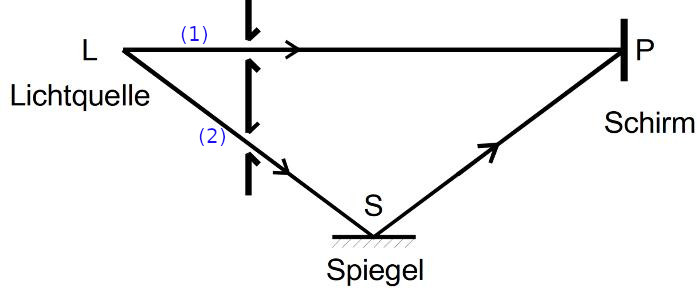
\includegraphics[scale=1.45]{Text/Bilder/kohaerenz.jpg}
  \caption{Interferenzerzeugung mit einer gewöhnlichen Lichtquelle \cite[]{sample}.}
  \label{fig:koh}
\end{figure}
Jedoch ist dabei zu beachten, dass Elektronen nur endliche Wellenzüge emittieren. Legt der Strahl $(2)$ aus Abbildung \ref{fig:koh} einen
viel größeren Weg als der dort abgebildete Strahl $(1)$ zurück, treffen Lichtstrahlen aus unterschiedlichen Emissionen aufeinder, wodurch sie nicht mehr kohären sind.
Dabei sind zwei Lichtstrahlen genau dann kohärent, wenn ihre Phasenverschiebung zeitlich kosntant bleibt.
Die Wegdifferenz mehrerer kohärenter Wellen wird dabei als Gangunterschied bezeichnet.
Für den maximalen Gangunterschied $\ell$ gilt:
\begin{equation}
  \ell = N\lambda
\end{equation}
\begin{center}
 \small {($ N \: \hat{=} \:\text{Maximale Anzahl der sichtbaren Maxima}$)}
\end{center}
%wegdifferenz
Die Forderung eines maximal möglichen Gangunterschied folgt ebenso aus dem Fourierschen Theorem. Dieses besagt, dass
ein Wellenzug endlicher Länge nicht monochromatisch sein kann, sondern ein Frequenz- und Wellenlängenspektrum besitzen muss.
Mit dem Frequenzsprektrum
\begin{equation}
  E(t)=\begin{cases}
  E_0\mathrm{e}^{-i\omega_0t} & \text{für} -\frac{\tau}{2}<t<\frac{\tau}{2}\\
  0 & \text{sonst}
  \end{cases}
\end{equation}
eines Wellenzuges kann mithilfe der Fouriertranformation und der Bildung des Betragsquadrates folgender Zusammenhang für die Intensität $I$ einer punktförmigen
Lichtquelle in Abhängigkeit der Kreisfrequenz $\omega$ gefunden werden:
\begin{equation}
  I(\omega)= 4 {E_0}^2 \frac{\sin(\omega-\omega_0)l}{(\omega-\omega_0)^2 2c} \text{.}
\end{equation}
In der Realität verfügen Lichtquellen jedoch über eine endliche Ausbreitung, wodurch sich der Kontrast des Interferenzmusters verschlechtert.
Dies kann nicht vermieden, jedoch reduziert werden. Dazu wird die Ausdehnung der Lichtquelle oder der zu betrachtende Winkelbereich möglichst gering gehalten.

\subsection{Das Michelson-Interferometer} \label{sec:MIF}
\begin{figure}[H]
  \centering
  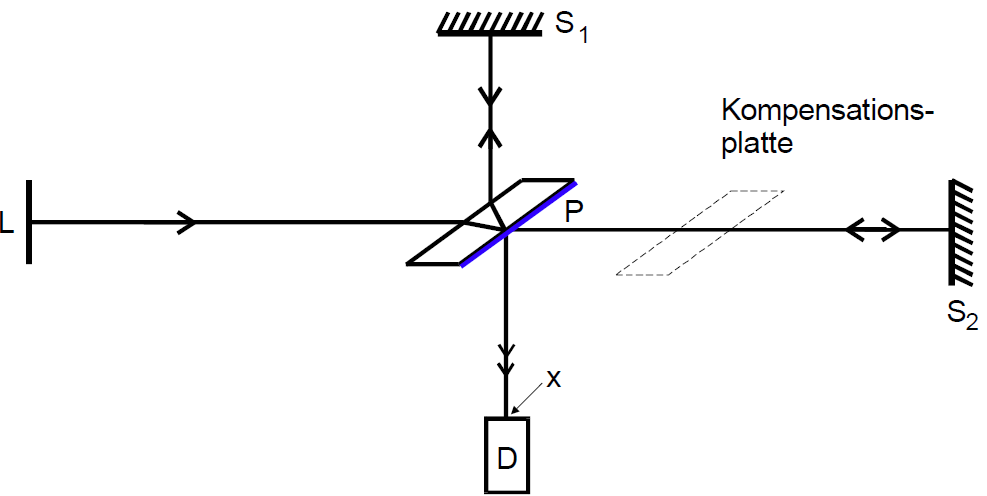
\includegraphics[scale=0.55]{Text/Bilder/schematischerAufbau.png}
  \caption{Prinzipieller Aufbau eines Michelson-Interferometers.
  $S_i \: \hat{=} \: \text{Spiegel}$, $P \: \hat{=} \: \text{semipermeabler Spiegel}$, $L \: \hat{=} \: \text{Lichtquelle}$, $D \: \hat{=} \: \text{Detektor}$ \cite[]{sample}}
  \label{fig:SA}
\end{figure}
Wie in Abbildung \ref{fig:SA} zu sehen ist, besteht das Michelson Interferometer aus einer Lichtquelle, zwei Spiegeln, einem Detektor, einem semipermeablen Spiegel und einer
Kompensationsplatte.
Licht aus der Lichtquelle fällt auf den semipermeablen Spiegel. Dieser ist im $\SI{45}{°}$-Winkel aufgestellt und spaltet den Strahl in zwei % zueinander kohärente
 Teilstrahlen auf.  Beide Strahlen werden, wie in Abbildung \ref{fig:SA} zu sehen, an einem Spiegel reflektiert und zum semipermeablen Spiegel zurückgeführt, an dem sie zum Detektor
reflektiert werden.
Um Interferenz beobachten zu können, muss der optische Wegunterschied kleiner als die Kohärenzlänge sein. Dies wird erreicht, wenn die Strecken $\overline{DS_1}$ und $\overline{DS_2}$ gleich groß sind.
Da der von $S_1$ kommende Strahl jedoch 3 mal den semipermeablen Spiegel durchläuft, während der von $S_2$ kommende Strahl dies nur 1 mal tut, muss letzterer zusätzlich eine Kompensationsplatte durchlaufen.
Diese hat dabei den selben Brechungsindex und Dicke wie der semipermeable Spiegel, womit beide Strahlen denselben optischen Weg durchlaufen.
Wird der Gangunterschied nun durch verschieben des Spiegels $S_1$ um den Abstand $\symup{\symup{\Delta}}d$  variiert, ändert sich der Gangunterschied. Daraufhin ändert sich das Interferenzbild.
Mit der Gleichung
\begin{equation}
  \lambda=\frac{2 \symup{\Delta} d}{z}
\end{equation}
lässt sich mithilfe der Wegdifferenz $\symup{\Delta} d$ und Maximalanzahl $z$ auf die Wellenlänge zurückführen.
Wird die optische Wegstrecke durch eine Veränderung des Brechungsindexes $\symup{\Delta} n$ verlängert, gilt folgender Zusammenahg für die Wellenlänge:
\begin{equation}
  \lambda=\frac{2b \symup{\Delta} n}{z}
\end{equation}
\begin{center}
 \small {($ b \: \hat{=} \:\text{Länge des Materials mit Brechungsindex $n+\symup{\Delta} n$}$)}
\end{center}
Dieser Fall ist in Abbildung \ref{fig:SA2} dargestellt.
\begin{figure}[H]
  \centering
  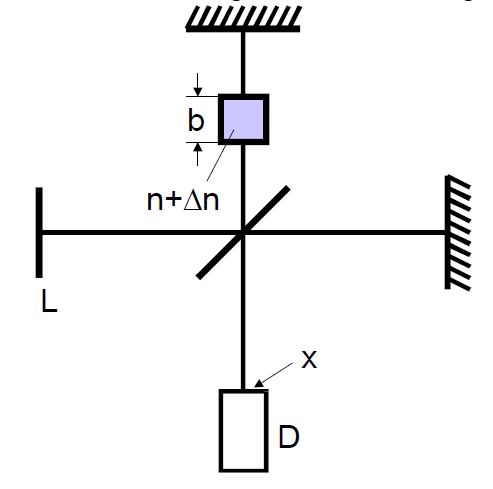
\includegraphics[scale=0.55]{Text/Bilder/schematischerAufbau2.png}
  \caption{Prinzipielle Versuchsordnung zur Messung kleiner Brechungsindexunterschiede mit dem Michelson-Interferometer \cite[10]{sample}.}
  \label{fig:SA2}
\end{figure}
Ebenso lässt sich zeigen, dass für den Brechungsindex der Zusammenhang
\begin{equation}
  n = \sqrt{1+f(\lambda)N}
\end{equation}
\begin{center}
 \small {($ N \: \hat{=} \:\text{Anzahl der zur Schwingung angeregten Moleküle}$)}
\end{center}
gilt, der sich mithilfe einer Taylor-Näherung mit
\begin{equation}
  n=1+\frac{fn}{2}
\end{equation}
nähern lässt. %jaja, doppelt gemoppelt, aber mir fällt nichts schöneres ein
Mithilfe der idealen Gasgleichung
\begin{equation}
  p V = R T
\end{equation}
\begin{center}
 \small {($ p \: \hat{=} \:\text{Druck}$, $ V \: \hat{=} \:\text{Volumen}$, $ T \: \hat{=} \:\text{Temperatur}$, $ p \: \hat{=} \:\text{Druck}$, $ R \: \hat{=} \:\text{Universelle Gaskonstante}$ )}
\end{center}
lässt sich durch Betrachtung von $p$ und $p'$ der Zusammenhang
\begin{equation}
  n(p_0,T_0)=1+\frac{Z\lambda}{2b}\frac{T}{T_0}\frac{p_0}{p-p'}
\end{equation}
aufstellen.
